\documentclass[a4paper]{article}
\usepackage[utf8]{inputenc}
\usepackage{tikz}
\usepackage{hyperref}
\usepackage{graphicx}
% \setlength{\parskip}{0.5em}
\usetikzlibrary{positioning, shapes.geometric}

%_______________________________________________________________
%                    Packages needed:
%_______________________________________________________________
\usepackage{tikz, adjustbox}
\usepackage[most]{tcolorbox}
\usepackage{xcolor}
\usepackage{wrapfig}
\newcommand*{\plogo}{\fbox{$\mathcal{PL}$}} % Generic dummy publisher logo
\usepackage[utf8]{inputenc} % Required for inputting international characters
\usepackage[T1]{fontenc} % Output font encoding for international characters
\usepackage{stix} % Use the STIX fonts
\usepackage[utf8]{inputenc}
\usepackage{xcolor}
\usepackage[explicit]{titlesec}
\usepackage{soul}
\usepackage[a4paper, margin=1in]{geometry}

%................................................................
%
%           Defining colors for sticky notes:
%_______________________________________________________________
% Yellow:
\definecolor{BgYellow}{HTML}{FFF59C}
\definecolor{FrameYellow}{HTML}{F7A600}
% Pink:
\definecolor{BgPink}{HTML}{EF6FA7}
\definecolor{FramePink}{HTML}{E5446E}
% Green:
\definecolor{BgGreen}{HTML}{C7D92D}
\definecolor{FrameGreen}{HTML}{89B23B}
% Blue:
\definecolor{BgBlue}{HTML}{45BEE9}
\definecolor{FrameBlue}{HTML}{31A8C9}
% White:
\definecolor{BgWhite}{HTML}{D8D8D8}
\definecolor{FrameWhite}{HTML}{7F7F7F}
% Brown:
\definecolor{BgBrown}{HTML}{8E7A45}
\definecolor{FrameBrown}{HTML}{6B5B32}
%................................................................
%
%                   Dummy text package:
%_______________________________________________________________
\usepackage{lipsum}
%................................................................
%
%                   NB command:
%_______________________________________________________________
\usepackage{contour}
\newcommand{\NB}{\contour{black}{\textbf{{\large\sffamily\color{red}NB}}}\textbf{\large\sffamily: }}
%................................................................
%
%               Defining Sticky note boxes:
%_______________________________________________________________
% Yellow Sticky Note (YStkyNote):
\newtcolorbox{YStkyNote}[1][]{%
    enhanced,
    before skip=2mm,after skip=2mm, 
    width=0.4\textwidth, % width of the sticky note
    boxrule=0.2mm,
    colback=BgYellow, colframe=FrameYellow, % Colors
    attach boxed title to top left={xshift=0cm,yshift*=0mm-\tcboxedtitleheight},
    varwidth boxed title*=-3cm,
    % The titlebox:
    boxed title style={frame code={%
        \path[left color=FrameYellow,right color=FrameYellow,
        middle color=FrameYellow]
        ([xshift=-0mm]frame.north west) -- ([xshift=0mm]frame.north east)
        [rounded corners=0mm]-- ([xshift=0mm,yshift=0mm]frame.north east)
        -- (frame.south east) -- (frame.south west)
        -- ([xshift=0mm,yshift=0mm]frame.north west)
        [sharp corners]-- cycle;
        },interior engine=empty,
    },
    sharp corners,rounded corners=southeast,arc is angular,arc=3mm,
    % The "folded paper" in the bottom right corner:
    underlay={%
        \path[fill=BgYellow!80!black] ([yshift=3mm]interior.south east)--++(-0.4,-0.1)--++(0.1,-0.2);
        \path[draw=FrameYellow,shorten <=-0.05mm,shorten >=-0.05mm,color=FrameYellow] ([yshift=3mm]interior.south east)--++(-0.4,-0.1)--++(0.1,-0.2);
        },
    drop fuzzy shadow, % Shadow
    fonttitle=\bfseries, 
    title={#1}
}
% Pink Sticky Note (PStkyNote):
\newtcolorbox{PStkyNote}[1][]{%
    enhanced,
    before skip=2mm,after skip=2mm, 
    width=0.4\textwidth, % width of the sticky note
    boxrule=0.2mm, 
    colback=BgPink, colframe=FramePink, % Colors
    attach boxed title to top left={xshift=0cm,yshift*=0mm-\tcboxedtitleheight},
    varwidth boxed title*=-3cm,
    % The titlebox:
    boxed title style={frame code={%
        \path[left color=FramePink,right color=FramePink,
        middle color=FramePink]
        ([xshift=-0mm]frame.north west) -- ([xshift=0mm]frame.north east)
        [rounded corners=0mm]-- ([xshift=0mm,yshift=0mm]frame.north east)
        -- (frame.south east) -- (frame.south west)
        -- ([xshift=0mm,yshift=0mm]frame.north west)
        [sharp corners]-- cycle;
        },interior engine=empty,
    },
    sharp corners,rounded corners=southeast,arc is angular,arc=3mm,
    % The "folded paper" in the bottom right corner:
    underlay={%
        \path[fill=BgPink!80!black] ([yshift=3mm]interior.south east)--++(-0.4,-0.1)--++(0.1,-0.2);
        \path[draw=FramePink,shorten <=-0.05mm,shorten >=-0.05mm,color=FramePink] ([yshift=3mm]interior.south east)--++(-0.4,-0.1)--++(0.1,-0.2);
        },
    drop fuzzy shadow, % Shadow
    fonttitle=\bfseries, 
    title={#1}
}
% Green Sticky Note (GStkyNote):
\newtcolorbox{GStkyNote}[1][]{%
    enhanced,
    before skip=2mm,after skip=2mm, 
    width=0.4\textwidth, % width of the sticky note
    boxrule=0.2mm,
    colback=BgGreen, colframe=FrameGreen, % Colors
    attach boxed title to top left={xshift=0cm,yshift*=0mm-\tcboxedtitleheight},
    varwidth boxed title*=-3cm,
    % The titlebox:
    boxed title style={frame code={%
        \path[left color=FrameGreen,right color=FrameGreen,
        middle color=FrameGreen]
        ([xshift=-0mm]frame.north west) -- ([xshift=0mm]frame.north east)
        [rounded corners=0mm]-- ([xshift=0mm,yshift=0mm]frame.north east)
        -- (frame.south east) -- (frame.south west)
        -- ([xshift=0mm,yshift=0mm]frame.north west)
        [sharp corners]-- cycle;
        },interior engine=empty,
    },
    sharp corners,rounded corners=southeast,arc is angular,arc=3mm,
    % The "folded paper" in the bottom right corner:
    underlay={%
        \path[fill=BgGreen!80!black] ([yshift=3mm]interior.south east)--++(-0.4,-0.1)--++(0.1,-0.2);
        \path[draw=FrameGreen,shorten <=-0.05mm,shorten >=-0.05mm,color=FrameGreen] ([yshift=3mm]interior.south east)--++(-0.4,-0.1)--++(0.1,-0.2);
        },
    drop fuzzy shadow, % Shadow
    fonttitle=\bfseries, 
    title={#1}
}
% Blue Sticky Note (BStkyNote):
\newtcolorbox{BStkyNote}[1][]{%
    enhanced,
    before skip=2mm,after skip=2mm, 
    width=0.4\textwidth, % width of the sticky note
    boxrule=0.2mm,
    colback=BgBlue, colframe=FrameBlue, % Colors
    attach boxed title to top left={xshift=0cm,yshift*=0mm-\tcboxedtitleheight},
    varwidth boxed title*=-3cm,
    % The titlebox:
    boxed title style={frame code={%
        \path[left color=FrameBlue,right color=FrameBlue,
        middle color=FrameBlue]
        ([xshift=-0mm]frame.north west) -- ([xshift=0mm]frame.north east)
        [rounded corners=0mm]-- ([xshift=0mm,yshift=0mm]frame.north east)
        -- (frame.south east) -- (frame.south west)
        -- ([xshift=0mm,yshift=0mm]frame.north west)
        [sharp corners]-- cycle;
        },interior engine=empty,
    },
    sharp corners,rounded corners=southeast,arc is angular,arc=3mm,
    % The "folded paper" in the bottom right corner:
    underlay={%
        \path[fill=BgBlue!80!black] ([yshift=3mm]interior.south east)--++(-0.4,-0.1)--++(0.1,-0.2);
        \path[draw=FrameBlue,shorten <=-0.05mm,shorten >=-0.05mm,color=FrameBlue] ([yshift=3mm]interior.south east)--++(-0.4,-0.1)--++(0.1,-0.2);
        },
    drop fuzzy shadow, % Shadow
    fonttitle=\bfseries, 
    title={#1}
}
% White Sticky Note (WStkyNote):
\newtcolorbox{WStkyNote}[1][]{%
    enhanced,
    before skip=2mm,after skip=2mm, 
    width=0.4\textwidth, % width of the sticky note
    boxrule=0.2mm,
    colback=BgWhite, colframe=FrameWhite, % Colors
    attach boxed title to top left={xshift=0cm,yshift*=0mm-\tcboxedtitleheight},
    varwidth boxed title*=-3cm,
    % The titlebox:
    boxed title style={frame code={%
        \path[left color=FrameWhite,right color=FrameWhite,
        middle color=FrameWhite]
        ([xshift=-0mm]frame.north west) -- ([xshift=0mm]frame.north east)
        [rounded corners=0mm]-- ([xshift=0mm,yshift=0mm]frame.north east)
        -- (frame.south east) -- (frame.south west)
        -- ([xshift=0mm,yshift=0mm]frame.north west)
        [sharp corners]-- cycle;
        },interior engine=empty,
    },
    sharp corners,rounded corners=southeast,arc is angular,arc=3mm,
    % The "folded paper" in the bottom right corner:
    underlay={%
        \path[fill=BgWhite!80!black] ([yshift=3mm]interior.south east)--++(-0.4,-0.1)--++(0.1,-0.2);
        \path[draw=FrameWhite,shorten <=-0.05mm,shorten >=-0.05mm,color=FrameWhite] ([yshift=3mm]interior.south east)--++(-0.4,-0.1)--++(0.1,-0.2);
        },
    drop fuzzy shadow, % Shadow
    fonttitle=\bfseries, 
    title={#1}
}
% Brown Sticky Note (BrStkyNote):
\newtcolorbox{BrStkyNote}[1][]{%
    enhanced,
    before skip=2mm,after skip=2mm, 
    width=0.4\textwidth, % width of the sticky note
    boxrule=0.2mm,
    colback=BgBrown, colframe=FrameBrown, % Colors
    attach boxed title to top left={xshift=0cm,yshift*=0mm-\tcboxedtitleheight},
    varwidth boxed title*=-3cm,
    % The titlebox:
    boxed title style={frame code={%
        \path[left color=FrameBrown,right color=FrameBrown,
        middle color=FrameBrown]
        ([xshift=-0mm]frame.north west) -- ([xshift=0mm]frame.north east)
        [rounded corners=0mm]-- ([xshift=0mm,yshift=0mm]frame.north east)
        -- (frame.south east) -- (frame.south west)
        -- ([xshift=0mm,yshift=0mm]frame.north west)
        [sharp corners]-- cycle;
        },interior engine=empty,
    },
    sharp corners,rounded corners=southeast,arc is angular,arc=3mm,
    % The "folded paper" in the bottom right corner:
    underlay={%
        \path[fill=BgBrown!80!black] ([yshift=3mm]interior.south east)--++(-0.4,-0.1)--++(0.1,-0.2);
        \path[draw=FrameBrown,shorten <=-0.05mm,shorten >=-0.05mm,color=FrameBrown] ([yshift=3mm]interior.south east)--++(-0.4,-0.1)--++(0.1,-0.2);
        },
    drop fuzzy shadow, % Shadow
    fonttitle=\bfseries, 
    title={#1}
}

% 
\definecolor{titleblue}{HTML}{2A202C}

\newbox\TitleUnderlineTestBox
\newcommand*\TitleUnderline[1]
  {%
    \bgroup
    \setbox\TitleUnderlineTestBox\hbox{\colorbox{titleblue}\strut}%
    \setul{\dimexpr\dp\TitleUnderlineTestBox-.3ex\relax}{.3ex}%
    \ul{#1}%
    \egroup
  }
\newcommand*\SectionNumberBox[1]
  {%
    \colorbox{titleblue}
      {%
        \makebox[2.5em][c]
          {%
            \color{white}%
            \strut
            \csname the#1\endcsname
          }%
      }%
    \TitleUnderline{\ \ \ }%
  }
\titleformat{\section}
  {\Large\bfseries\sffamily\color{titleblue}}
  {\SectionNumberBox{section}}
  {0pt}
  {\TitleUnderline{#1}}
\titleformat{\subsection}
  {\large\bfseries\sffamily\color{titleblue}}
  {\SectionNumberBox{subsection}}
  {0pt}
  {\TitleUnderline{#1}}


\begin{document}
    \begin{titlepage}
        \raggedleft
        \rule{1pt}{\textheight}
        \hspace{0.05\textwidth}
        \parbox[b]{0.75\textwidth}{
            {\Huge\bfseries \textcolor[HTML]{2A202C}{Backend Developer}\\[0.5\baselineskip] \textcolor[HTML]{2A202C}{Roadtrip}}\\[2\baselineskip]
            {\large\textit{\textcolor[HTML]{2A202C}{Random Collection of Knowledge}}}\\[4\baselineskip]
            {\Large\textsc{\textcolor[HTML]{2A202C}{Eduardo Cardenaz}}}
            
            \vspace{0.5\textheight}
        }
    \end{titlepage}

    \thispagestyle{empty} % Optional: removes header and footer on the new page
    \vspace*{\fill}
    \begin{center}
        \Huge Part I: Basics
    \end{center}
    \vspace*{\fill}
    \newpage

    \section{APIs}
    \paragraph*{Application Programming Interface (API)} An API is basically an intermediary that allows two applications to talk to each other. 

    It's useful to think of API communication in terms of requests and responses between a client and a server. The application submitting the request is the client, and the server provides the response.

    \paragraph{API Specification} Is a document or standard that describes how to build or how to use an API. A system that meets this standard its said to be \textit{implementing} or \textit{exposing} an API. The term API can refer to both the implementation and the specification.

    \subsection{RESTful APIs}
    

    REST stands for Representational State Transfer, and it's an architectural style for designing networked applications. A RESTful API (Application Programming Interface) adheres to the principles of REST.


    "The design rationale behind the Web architecture can be described by an architectural style consisting of the set of constraints applied to elements within the architecture." \href{https://ics.uci.edu/~fielding/pubs/dissertation/rest_arch_style.htm}{source}

    To understand REST, we'll be expanding and building on top of each constraint that composes this architecture.

    Violating any constraint other than Code on Demand means that the service is not strictly RESTful.

    
    \subsubsection{Uniform Interface}
    \paragraph{Resource Based}
    Individual resources are identified using URIs as resource identifiers. The resources themselves are conceptually different from the \textit{representation} that is returned to the client. For example, the server doesn't return its database but rather some HTML, JSON or XML that represents some database records.

    \paragraph{Manipulation of Resources Through Representations} When a client holds a representation of a resource given by the server, including any metadata attached to it, it should have enough information to modify or delete said resource on the server, given it has the right permissions. 

    \paragraph{Self-Descriptive Messages} Each message includes all the necessary information to describe how to handle that message. 

    
    \subsubsection{Client-Server} Separation of Concerns is the principle behind this constraint. By separating the user interface (UI) concerns from the data storage concerns, we improve the portability of the UI across multiple platforms.
    

    \subsubsection{Stateless} This constraint stablish that the interaction between the client and the server must be stateless in nature, by that, meaning that any request made by the client must contain all the necessary information so that the server can understand the request. It shall not take advantage of any stored context. 
    
    \paragraph{Stateless} Imagine that you're buying coffee at a shop. Each time you want to order a coffee you need to tell the cashier exactly what you want and how you want it. The cashier doesn't remember you or what you ordered the last time you went there. Each visit is like starting from scratch. 

    \paragraph{Stateful} The cashier remembers you and remember what you usually ask for as you're a frequent client. So, you could say 'the usual' and they'd know exactly what you want.

    \subsubsection{Cacheable} Clients should can cache responses. Responses must, implicitly or explicitly, define themselves as cacheable or not. Clients should be able to negotiate wether to cache or not to prevent reusing stale or inappropriate data in response to further requests.


    \subsubsection{Layered System} A client cannot tell whether its connected to the main server or an intermediary along the way. The layered system style allows an application to be composed of hierarchical layers by constraining component behavior such that each component can't see beyond the immediate layer with which they are interacting.

    \subsubsection{Code on Demand} This is a kind-of unique thing about RESTful systems. Code on Demand is optional. Basically means that a server can temporarily extend functionality to a client by transferring logic to the client. As an example, a request can return client-side scripts such as Javascript code.


    \subsection{JSON APIs}
    \subsection{SOAP APIs}
    \subsection{GraphQL APIs}
    \subsection{gRPC APIs}
    
    \subsection{Authentication \& Authorization}
    \paragraph*{Authentication} is the process that an individual, process or system goes through to \textbf{prove} their identity before gaining access to digital systems.

    \paragraph*{Authorization} is the process of determining whether a user, system or application has the necessary permissions to perform a particular action within a system. 

    \paragraph*{API Authentication} validates the identity of the client attempting to make a connection by using an authentication protocol. The protocol sends the credentials from the remote client requesting access to the server for verification, usually the credentials are in either plain text or some form of encrypted format.

    \subsubsection{Session Authentication} 
    
    \paragraph*{Session} A session, refers to a temporary, stateful interaction between a user and a server. 
    A session, is a period of interaction between a user an a server, during which the user's actions and data are temporarily stored and managed by the server. 

    \begin{itemize}
        \item \textbf{Duration}: A session begins when the user logs into the server and ends when they log out, or after a period of inactivity. 
        \item \textbf{Session Data}: During the sessions, the server stores information relevant to the user's interaction, such as their authentication status, user ID, preferences, etc.
        \item \textbf{Session ID}: To uniquely identify each sessions, the server assigns a session identifier. This session id is used to to associate the Session Data with the User
    \end{itemize}

    \paragraph*{Example} When you log in (authenticate) into a web application, the server creates a session and then keeps track of it itself. Then it creates a Session ID and gives it to you, subsequently, the client (you) pass this Session ID to the server with each request. Then, the Server looks this Session ID up in its Session Log, and if it finds it, it knows who you are and what you're allowed to do.

    How the client passes the Session ID to the server, depends on the implementation, but it's usually done through Cookies.


    \subsubsection{JWT}

    \paragraph*{JWT} or JSON Web Token, is a compact, URL-Safe means of representing claims between two parties. The claims in a JWT are encoded as JSON objects.

    A JWT consists of three parts:

    \begin{itemize}
        \item \textbf{Header}: Contains the type of token and the signing algorithm being use. (e.g. HMAC SHA256, or RSA).
        \item \textbf{Payload}: Contains the Claims. Claims are statements about an entity (typically the user) and additional data.
        \item \textbf{Signature}: The signature is created by taking the combined encoded header and payload, and signing it using the algorithm specified in the header and a secret key or private key.
    \end{itemize}

    \paragraph*{Claims} In the context of JWT, claims refer to pieces of information that are included in the token. These pieces of information are \textbf{statements} about an entity. Claims are stored in the payload part of the JWT.

    There are three types of Claims.
    
    \begin{itemize}
        \item \textbf{Registered Claims}: These are part of a set of predefined claims which are not mandatory but recommended to provide a set of useful, interoperable claims, like:
        \begin{itemize}
            \item \textbf{iss} (issuer): Identifies the principal that issued the JWT.
            \item \textbf{sub} (subject): Identifies the principal that is the subject of the JWT.
            \item \textbf{aud} (audience): Identifies the recipients that the JWT is intended for.
            \item \textbf{exp} (expiration time): Identifies the expiration time on or after which the JWT must not be accepted for processing.
            \item \textbf{nbf} (not before): Identifies the time before which the JWT must not be accepted for processing.
            \item \textbf{iat} (issued at): Identifies the time at which the JWT was issued.
            \item \textbf{jti} (JWT ID): Provides a unique identifier for the JWT.
        \end{itemize}
        \item \textbf{Public Claims}: They can be defined by developers to include custom information. These claims can be used publicly, meaning that they can be understood by anyone who processes the JWT.
        \item These are custom claims created to share information between parties that agree on using them. They are neither registered nor public claims, and they are meant to be used within a specific context between the parties involved.
    \end{itemize}


    \subsubsection{Basic Auth}
    \subsubsection{Token Auth}
    \subsubsection{OAuth}
    \subsubsection{Cookie Based}
    \subsubsection{OpenID \& SAML}

    \section*{HTTP}

    \paragraph{Hypertext Transfer Protocol (HTTP)} Is a protocol for fetching resources over the internet. It is the foundation of the Web and its a client-server protocol. Clients, usually a web browser, and servers communicate by exchanging messages. The messages send by the client are called Requests and the messages sent by the server are called Responses.

    \paragraph*{Client-Server Architecture} HTTP operates on a client-server model where the client (usually a web browser) send a request to the server, and the server responds with the requested resource (e.g. an HTML page, image, or JSON data)

    \paragraph*{Stateless Protocol} Each HTTP request from a client to a server is independent; it carries all the information the server needs to fulfill the request. This stateless nature simplifies server design bc it doesn't need to retain information about previous requests.

    \subsection{HTTP Methods \& Status Codes}
        \subsubsection{HTTP Methods}
            \paragraph{GET} Requests a representation of a specified resource. GET requests should only retrieve data.
            \paragraph{POST} Submits data to be processed to a specified resource, often causing a change in state or side effects on the server.
            \paragraph{PUT} Replaces all current representations of the target resource with the request payload.
            \paragraph{DELETE} Removes the specified resource.
            \paragraph{PATCH} Applies partial modifications to a resource.
        \subsubsection{HTTP Status Codes} Most common status codes.
            \paragraph{1xx Informational}
            \paragraph{2xx Success}

            \begin{itemize}
                \item 200 OK: The request has succeeded.
                \item 201 Created: The request succeeded, and a new resource was created as a result. This is typically the response for a POST request.
                \item 204 No Content: The request was successful, but there is no content tos end in the response.
            \end{itemize}

            \paragraph{3xx Redirection} 

            \begin{itemize}
                \item 301 Moved Permanently: The requested resource has been permanently moved to a new location.
                \item 302 Found: The requested resource has been temporarily moved to a new location.
            \end{itemize}

            \paragraph{4xx Client Errors}

            \begin{itemize}
                \item 400 Bad Request: The server cannot process the request due to a client error.
                \item 401 Unauthorized: The client must authenticate itself to get the requested response.
                \item 403 Forbidden: The client does not have permission to access the requested resource.
                \item 404 Not Found: The server cannot find the requested resource.
            \end{itemize}

            \paragraph{5xx Server Errors}

            \begin{itemize}
                \item 500 Internal Server Error: The server has encountered a situation it doesn't know how to handle.
                \item 502 Bad Gateway: The server, while acting as a gateway or proxy, received an invalid response from the upstream server. Meaning the server is down or being upgraded.
                \item 503 Service Unavailable: The server is not ready to handle the request. Common causes are a server that is down for maintenance or that is overloaded.
                \item 504 Gateway Timeout: The server, while acting as a gateway or proxy, did not receive a timely response from the upstream server.
            \end{itemize}


    \subsection{Common HTTP Headers}

    HTTP Headers are key-value pairs sent between the client and the server in an HTTP request or response. They provide essential information about the request, the resposne, and the data being transferred. Examples of the most common headers include:

        \paragraph{General Headers}

        \begin{itemize}
            \item \textbf{Cache-Control}: Specifies directives for caching mechanisms in both requests and responses. Examples of directives include \textit{no-cache}, \textit{no-store}, \textit{max-age}, and \textit{must-revalidate}. 
            \item \textbf{Connection}: Controls whether the network connection stays open after the current transaction finishes. Examples of values include \textit{keep-alive} and \textit{close}. Keep-alive allows the connection to be reused for multiple requests. Close forces the connection to close after the current request.
            \item \textbf{Date}: The date and time at which the message was sent.
        \end{itemize}

        \paragraph{Request Headers}

        \begin{itemize}
            \item \textbf{Accept}: Specifies the media types that the client can understand. The server should respond with one of these media types. Example values include \textit{text/html}, \textit{application/json}, and \textit{image/png}.
            \item \textbf{Accept-Encoding}: Specifies the encoding algorithms that the client can understand. The server should respond with one of these encoding algorithms. Example values include \textit{gzip}, \textit{deflate}, and \textit{br}.
            \item \textbf{Accept-Language}: Specifies the natural languages that the client can understand. The server should respond with one of these languages. Example values include \textit{en-US}, \textit{es}, and \textit{fr}.
            \item \textbf{Authorization}: Contains credentials for authenticating the client with the server.
            \item \textbf{User-Agent}: Contains information about the client making the request. This can include the client's operating system, browser, and version.
            \item \textbf{Content-Type}: Specifies the media type of the data being sent in the request.
        \end{itemize}

        \paragraph{Response Headers}

        \begin{itemize}
            \item \textbf{Content-Type}: Specifies the media type of the data being sent in the response.
            \item \textbf{Content-Length}: Specifies the length of the response body in octets (8-bit bytes).
            \item \textbf{Set-Cookie}: Sets a cookie in the client's browser. Cookies are used to store information about the client's session.
            \item \textbf{Location}: Specifies the URL to redirect the client to. This is often used in 3xx redirection responses.
            \item \textbf{WWW-Authenticate}: Specifies the authentication method that the client must use to access the resource.
        \end{itemize}


        \subsubsection{Content-Type} This header is a critical component that indicates the media type of the resource being sent. It tells the client or the server how to interpret the data in the body of the request or response. 

        The \textit{Content-Type} header consists of: 

        \begin{itemize}
            \item \textbf{Media Type}: The type of data being sent (e.g., text, image, application).
            \begin{itemize}
                \item \textit{text}: Represents textual information. Examples include HTML, CSS, and plain text.
                \item \textit{image}: Represents image data. Examples include PNG, JPEG, and GIF.
                \item \textit{application}: media types are used to denote formats that are usually processed by applications rather than directly read by humans. These types often require specific software to interpret or manipulate the data.
            \end{itemize}
            \item \textbf{Subtype}: The specific format of the data (e.g., HTML, JSON, PNG).
            \item \textbf{Optional Parameters}: Additional information about the media type, often specifying the character encoding (e.g., charset=UTF-8).
        \end{itemize}

        \paragraph{application/x-www-form-urlencoded} This is the default encoding for form data. It encodes form fields as key-value pairs, with special characters replaced by escape sequences. This encoding is commonly used in HTML forms and URL query strings. Note that the space character is encoded as \textit{\%20} or the plus sign (\textit{+}).

        \begin{verbatim}
            name=John+Doe&age=25
        \end{verbatim}

        \paragraph{application/json} Commonly used in API requests and responses to transfer JSON data. 

        \begin{verbatim}
            {
                "name": "John Doe",
                "age": 25
            }
        \end{verbatim}


        \paragraph{application/xml} Used to transfer XML data.

        \begin{verbatim}
            <person>
                <name>John Doe</name>
                <age>25</age>
            </person>
        \end{verbatim}



        \subsubsection{Content-Length} This headers specifies the size of the body of the request or response, measured in bytes. It is used by the client and server to understand the exact size of teh content being sent or received.

        \subsubsection{User-Agent} This headers provides a way to identify the client software that is making the request. This ehader contains a string that provides details about the user agent (browser, application, or other software) and the operating system it is running on. This information can be used by the server for various purposes, such as content negotiation, analytics and logging. 

        \subsubsection{Authorization} This header is used to proved credentials that atuhenticate the client to the server. This header allows the server to verify the identity of the client and grant acces to protected resources. The header supports various authentication schemes. 

        \begin{itemize}
            \item Basic Authentication: The client sends a base64-encoded username and password separated by a colon. The server decodes the credentials and verifies them against a user database.
            \item Bearer Token: The client sends a token that was previously obtained from the server. The server validates the token to authenticate the client.
            \item Digest Authentication: The client sends a hashed value of the username, password, and other information. The server verifies the hash to authenticate the client.
            \item OAuth: The client sends an access token that was previously obtained from an OAuth server. The server validates the token to authenticate the client.
            \item API Key: The client sends an API key that was previously obtained from the server. The server validates the key to authenticate the client.
            \item JWT: The client sends a JSON Web Token (JWT) that was previously obtained from the server. The server validates the token to authenticate the client.
        \end{itemize}

        Usually, the authorization header is in the format \textit{Authorization : <type> <credentials>} for example:

        \begin{verbatim}
            Authorization: Bearer eyHstOSkasd...
        \end{verbatim}


        \subsubsection{Cache-Control}
        \subsubsection{Cookie}
        \subsubsection{Set-Cookie}
        \subsubsection{Accept}
        \subsubsection{Accept-Encoding}
        \subsubsection{Host}
        \subsubsection{Referer}

    \subsection{Unicode \& Character Encoding}
        \paragraph{UTF-8}
        \paragraph{ISO-8859-1}
        \subsubsection{URL Encoding}
        
    \subsection{CORS}
        \paragraph{Origins}
        \paragraph{Headers}
        \paragraph{Methods}
        \paragraph{Credentials}
        \paragraph{Preflight Requests}
        
    \subsection{WebSockets}
        \paragraph{Protocol}
        \paragraph{Handshake}
        \paragraph{Frames}


        
    \subsection{HTTP Versions}
        \paragraph{HTTP/1.1}
        \paragraph{HTTP/2}
        \paragraph{HTTP/3}
        
    \subsection{HTTPS}
        \paragraph{TLS/SSL}
        \paragraph{Certificates}
        \paragraph{Handshake}

    \subsection{HTTP Cookies}
        \paragraph{Creation}
        \paragraph{Attributes}
        \paragraph{SameSite}
        \paragraph{Secure}
        \paragraph{HttpOnly}
    
    \section{Networking and Shit}
    \subsection{The OSI Model}

    \paragraph{The Open Systems Interconnection model} is a conceptual framework used to understand and implement standardized network protocols in seven layers. Each layer serves a specific function and communicates with the layers directly above and below it.

    \paragraph{IP Addresses} Unique identifier assigned to each device connected to a network. It allows devices to locate and communicate with each other.

    \begin{itemize}
        \item Public IP: Used on the internet.
        \item Private IP: Used within private networks (e.g., home or office)
    \end{itemize}

    \paragraph*{Ports} A port is a logical endpoint for communication, used to distinguish different types of network services running on the same IP address (device). 

    \begin{itemize}
        \item Well-Known Ports (0-1023): Assigned to widely used services and protocols.
        \item Registered Ports (1024-49151): Assigned by IANA for specific services. 
        \item Dynamic/Private Ports (49152-65535): Used for dynamic or temporary purposes.
    \end{itemize}

    \paragraph{Domain Name System (DNS)} The DNS translates human-readable domain names (e.g., www.example.com) into IP addresses that computers use to identify each other on the network.




    \subsubsection{Application Layer} It s the topmost layer of the OSI model. It serves as the interface between the network services and the end-user applications. This layer provides the necessary protocols and functionalities for application to communicate over the network, enabling end-users to interact with networked systems.

    \paragraph{Key Functions}

    \begin{itemize}
        \item Network Services: Provides services like file transfers, email, remote login and web browsing.
        \item Data representation: Ensures data is presented in a readable format.
        \item Communication: Facilitates communication between software applicaitons and network services.
    \end{itemize}

    \paragraph{Common Protocols}

    \begin{itemize}
        \item HTTP (Hypertext Transfer Protocol): Used for web browsing. Usually runs on port 80.
        \item HTTPS: Secure version of HTTP, using SSL/TLS encryption. Usually runs on port 443.
        \item FTP (File Transfer Protocol): Used for transferring files between systems. Usually runs on port 21.
        \item SMTP (Simple Mail Transfer Protocol): Used for sending emails. Usually runs on port 25.
        \item DNS (Domain Name System): Translates domain names to IP addresses. Usually runs on port 53.
    \end{itemize}

    \paragraph*{Example Scenario} Accessing a Website.
    
    \begin{enumerate}
        \item URL Input: You enter `www.example.com` in your browser.
        \item DNS Lookup: the browser send a DNS query to find the IP address of `www.example.com`. The DNS server replies with `93.184.216.34`
        \item Sending a Request: The browser sends an HTTP request to `93.184.216.34` on port 80.
        \item Server Response: The web server listens on port 80, processes the request, and sends back the webpage content.
        \item Receiving Data: The browser receives the data and renders the webpage for you to view.
    \end{enumerate}

    \subsubsection{Presentation Layer} The Presentation Layer is the sixth layer of the OSI model. It acts as a translator between the application layer and the lower layers of the OSI model. This layer is responsible for the syntax and the semantics of the data being transmitted, ensuring that the data is readable by the receiving system.

    \paragraph{Key Functions}

    \begin{itemize}
        \item Data Translation: Converts data both incoming to the appplication and outgoing from the application into a format that can be sent over the network.
        \item Data Encryption and Decryption: Encrypts data before it is sent over the network to ensure secure comms.
        \item Data Compression: Compresses and decompresses the data to reduce the size of the data being transmitted.
        \item Serialization and Deserialization: Converts data into a format that can be stored or transmitted and then converts it back to its original form.
    \end{itemize}

    \paragraph*{Common Protocols}

    \begin{itemize}
        \item SSL/TLS: Secure Sockets Layer and Transport Layer Security are protocols used to encrypt data transmitted over the network. Most commonly used for HTTPS.
        \item ASCII: American Standard Code for Information Interchange is a character encoding standard used for text files in computers and other devices.
        \item JPEG: Joint Photographic Experts Group is a standard for compressing images.
    \end{itemize}

    This layers is also able to provide encryption and compression if the application layer ask it to do so.


    \subsubsection{Session Layer} The Session Layer is the fifth layer of the OSI model. It is the responsible for managing and controlling the dialogs (sessions)  between two devices. This layer establishes, maintains, and terminates connections between applications, ensuring that the data is properly synchronized and delivered.

    \paragraph{Common Protocols}

    \begin{itemize}
        \item NetBIOS: Network Basic Input/Output System is a protocol used for communication between computers on a local area network.
        \item PPTP: Point-to-Point Tunneling Protocol is used to create a virtual private network (VPN) over the internet.
        \item RPC: Remote Procedure Call is a protocol that allows a computer program to cause a subroutine or procedure to execute in another address space.
    \end{itemize}

    \subsubsection{Transport Layer}

    The Transport Layer is the fourth layer of the OSI model. It is responsible for end-to-end communication between the source and destination devices. This layer ensures that data is delivered error-free, in sequence, and without loss or duplication.

    \paragraph{Key Functions}
    
    \begin{itemize}
        \item Segmentation and Reassembly: Breaks down large data into smaller segments for transmission and reassembles them at the destination.
        \item Error Detection and Correction: Detects errors in the data and retransmits it if necessary.
        \item Flow Control: Manages the flow of data between devices to prevent data loss due to congestion.
    \end{itemize}

    \paragraph{Common Protocols}
    
    \begin{itemize}
        \item TCP (Transmission Control Protocol): Provides reliable, connection-oriented communication between devices. It ensures that data is delivered in the correct order and without errors.
        \item UDP (User Datagram Protocol): Provides connectionless communication between devices. It is faster than TCP but does not guarantee delivery or order of data.
    \end{itemize}

    \subsubsection{Network Layer}

    The Network Layer is the third layer of the OSI model. It is responsible for routing data from the source to the destination device. This layer determines the best path for data to travel and handles addressing, packet forwarding, and routing.

    \paragraph{Key Functions}

    \begin{itemize}
        \item Logical Addressing: Assigns logical addresses (IP addresses) to devices on the network.
        \item Routing: Determines the best path for data to travel from the source to the destination device.
        \item Packet Forwarding: Forwards data packets from one device to another based on the destination address.
    \end{itemize}

    \paragraph{Common Protocols}

    \begin{itemize}
        \item IP (Internet Protocol): Provides logical addressing and routing of data packets between devices on the network.
        \item ICMP (Internet Control Message Protocol): Used for error reporting and diagnostic functions in IP networks.
        \item ARP (Address Resolution Protocol): Maps IP addresses to MAC addresses on a local network.
        \item DHCP (Dynamic Host Configuration Protocol): Assigns IP addresses to devices on a network automatically.
    \end{itemize}


    \subsubsection{Data Link Layer}

    Defines the format of data on the network. 

    \subsubsection{Physical Layer}

    Defines the physical connection between devices. Transmits raw bit stream over the physical medium.


    \subsection{TCP/IP}
    \subsubsection{Transmission Control Protocol (TCP)} Is a network protocol that lets two host connect and exchange data streams. TCP guarantees that the packages and data that are sent, come in the same order as they were sent. 

    TCP is a connection-oriented protocol, meaning that it establishes a connection between the two hosts before sending data. It also ensures that the data is delivered error-free and in the correct order.

    \paragraph{Connection-Oriented Communication} TCP uses a three-way handshake to establish a connection between the two hosts. The three steps are:

    \begin{enumerate}
        \item SYN (Synchronize): Device A (the client) wants to start a conversation with Device B (the server).
        \item SYN-ACK (Synchronize-Acknowledge): The server responds with a SYN-ACK packet to acknowledge the connection request.
        \item ACK (Acknowledge): The client sends an ACK packet to confirm the connection.
    \end{enumerate}

    When it wants to terminate a connection, it uses a four-way handshake.

    \begin{enumerate}
        \item FIN (Finish): The client sends a FIN packet to the server to close the connection.
        \item ACK: The server responds with an ACK packet to acknowledge the request.
        \item FIN: The server sends a FIN packet to the client to close the connection.
        \item ACK: The client responds with an ACK packet to acknowledge the request.
    \end{enumerate}

    \paragraph*{Datagrams} Are the basic unit of information passed across the internet. They are packets of data that are sent and received over a network. 

    A datagram is a self-contained, independent packet of data that is sent over a network. It contains the source and destination addresses, as well as the data being transferred.

    \paragraph*{Internet Protocol (IP)} Is the principal communications protocol in the Internet protocol suite for relaying datagrams across network boundaries. Its routing function enables internetworking, and essentially establishes the Internet.





    \subsection{UDP}
    \subsection{DNS}

    \newpage
    \section{Caching}
    \subsection{Client Side}
    \subsection{Server Side}
    \subsection{Content Delivery Network (CDN)}
    \subsection{Redis}
    \subsection{Memcached}

    \newpage
    \section{Web Security}
    \subsection{Hashing Algorithms}
    \subsection{API Security Best Practices}

    \newpage
    \section{Testing}
    \subsection{Unit Testing}
    \subsection{Integration Testing}
    \subsection{Functional Testing}
    
    \newpage
    \section{CI/CD}
    
    \newpage
    \section{Databases}
    \subsection{Database Indexes}
    \subsection{Sharding Strategies}
    \subsection{CAP Theorem}
    \subsection{Data Replication}
    \subsection{ACID vs BASE}
    \subsection{Transactions}
    \subsection{N+1 Problem}
    \subsection{Normalization}
    \subsection{Failure Modules}
    \subsection{Profiling performance}
    
    
    \newpage
    \section{Software Design \& Architecture}
    \subsection{Design and Development Principles}
    \subsubsection{Separation of Concerns}
    \subsubsection{Reusability}
    \subsubsection{Keep It Simple Stupid (KISS)}
    \subsubsection{Don't Repit Yourself (DRY)}
    \subsubsection{Scalability}
    \subsubsection{Security}

    \subsection{GOF Design Patterns}
    \subsection{Domain Driven Design}
    \subsection{CQRS}
    \subsection{Event Sourcing}

    \newpage
    \section{Architectural Patterns}
    \subsection{Load Balancer}
    \subsection{Monolithic Apps}
    \subsection{Microservices}
    \subsection{SOA}
    \subsection{Serverless}
    \subsection{Service Mesh}
    \subsection{Twelve Factor App}

    \newpage
    \section{Message Brokers}
    \subsection{RabbitMQ}
    \subsection{Kafka}

    \newpage
    \section{Containerization Vs Virtualization} 
    \subsection{LXC}
    \subsection{Docker}
    \subsection{Kubernetes}
    \subsection{Elasticsearch}
    \subsection{Solr}


    \newpage
    \section{Web Servers}
    \subsection{Server Sent Events}
    \subsection{WebSockets}
    \subsection{Long Polling}
    \subsection{Short Polling}

    \newpage
    \section{GraphQL}
    \subsection{Apollo}

    \newpage
    \section{NoSQL Databases}
    \subsection{Document DBs - MongoDB}
    \subsection{Time Series - InfluxDB}
    \subsection{Realtime - Firebase}
    \subsection{Column DBs - Cassandra}
    \subsection{Key Value - Redis}
    \subsection{Graph DBs - Neo4j}

    \newpage
    \section{Building for Scale}
    \subsection{Difference + Usage}
    \subsection{Mitigation Strategies}


    \newpage

    \thispagestyle{empty} % Optional: removes header and footer on the new page
    \vspace*{\fill}
    \begin{center}
        \Huge Part II: Infraestructure Knowledge
    \end{center}
    \vspace*{\fill}
    \newpage


    \section{Go Programming Language}
    \subsection{}
    \subsection{}

    \newpage
    \section{Networking and Protocols}
    \subsection{}
    \subsection{}

    \newpage
    \section{Docker}
    \paragraph{Container} A container is a standard unit of software that packages up code and all its dependencies so the application runs quickly and reliably from one computing environment to another.

    A container is a way to package our applications including all the dependencies that it needs, including its configuration files. This makes them portable. Making development and deployment much faster. 

    \paragraph*{Image} A Docker Image is a lightweight, standalone, executable package of software that includes everything needed to run an application: code, runtime, system tools, system libraries and settings.

    An image is a packaging containing all the dependencies and the code. This is what's gonna be shared. Finally a container is an image we configured which its going to have all the dependencies running, alongside with environment variables, etc. A container, is basically layers upon layers of images, where usually the bottom layer is a Linux image. 

    A container is an instance of an image.

    \subsection{Virtualization}

    At its core, Docker is a virtualization tool. 

    \paragraph*{Virtualization} Is the process of creating a virtual version of something, such as an operating system, a server, a storage device or network resources. 

    \paragraph{Host} Being the physical machine that runs the virtualization software.

    \paragraph{Guest} The virtual machine or OS that runs on the host.
    

    \paragraph{Layers of Virtualization} The concept of virtualization is based on three layers.
    \begin{itemize}
        \item \textbf{Hardware}: Where the physical hardware is located. 
        \item \textbf{Kernel}: The kernel is the core of the operating system. It's the bridge between the hardware and the software.
        \item \textbf{Application}: This is your software, the applications you run on your computer.
    \end{itemize}

    \paragraph{A Virtual Machine (VM)} is a software that emulates a physical computer. It creates a virtualized environment that behaves like a separate computer. When you run a VM, the Kernel and the Application layers are what's being virtualized.

    As you may realize, this is very resource intensive.

    \paragraph*{Docker}, on the other hand, lives on the Application layer. It doesn't virtualize the hardware, nor the kernel. It just virtualizes the application. This makes it much more lightweight than a VM.


    \begin{figure}[h]
        \centering
        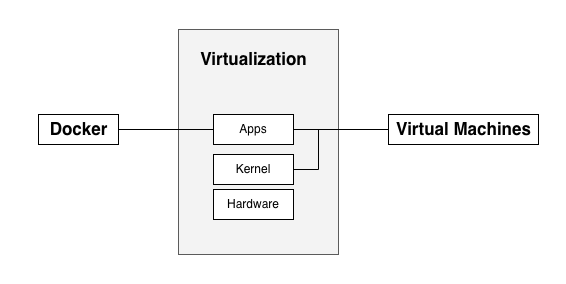
\includegraphics[width=0.5\textwidth]{img/docker-vs-vms.png}
        \caption{Docker vs VMs}
        \label{fig:my_label}
    \end{figure}

    \paragraph{Types of Virtualization} Exists three types of virtualization:
    \begin{itemize}
        \item \textbf{Para-Virtualization}: In para-virtualization, the host is trying to give the guest most of their hardware. 
        \item \textbf{Partial Virtualization}: Where some components of the host's hardware are virtualized and given to the guest.
        \item \textbf{Full Virtualization}: In full virtualization, the guest is given a full copy of the host's hardware.
    \end{itemize}

    For each of this cases, Docker is going to be superior, as Docker uses the kernel of the host directly.

    \subsection{Docker Network}

    \paragraph{Network} A Network in simple terms is a group of two or more devices that can communicate with each other either physically or virtually.

    \paragraph*{Docker Network} The Docker Network  is a virtual network created by Docker to enable communication between Docker Containers. Container Networking refers to the ability for containers to connect to and communicate withe ach other, or to non-Docker workloads.

    Containers have networking enabled by default, and they can make outgoing connections. A container has no information about what kind of network it's attached to, or whether their peers are also Docker workloads or not. 

    \paragraph*{Port Mapping} is a way to allow traffic to flow from the outside world into a container. Since containers are isolated environments, if you want to access a web application inside a container from your web browser, you need to map the port on which the application is running inside the container to a port on the host machine.

    \begin{figure}[h]
        \centering
        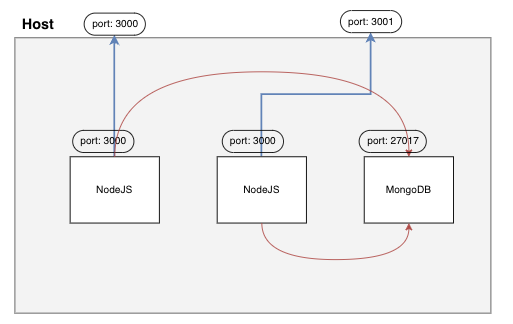
\includegraphics[width=0.5\textwidth]{img/docker-port-mapping.png}
        \caption{Docker Port Mapping}
        \label{fig:docker-port-mapping}
    \end{figure}

    As per the figure above, the Node JS container is running on port 3000. To access this container from the host machine, we need to map the port 3000 of the container to a port on the host machine. In this case, we're mapping the port 3000 of the container to the port 3000 of the host machine. 

    Usually, you would find that in cases where you have multiple containers running on the same port, you would map the port of the container to a different port on the host machine. So, if you have two containers with Node JS each with a web application running on port 3000, you would map the port of the first container to port 3000 of the host machine, and the port of the second container to port 3001 of the host machine. Although this is not mandatory, it's a good practice to avoid conflicts.




    \subsection{}
    \subsection{}
    
    \newpage
    \section{Amazon Web Services}
    \subsection{}
    \subsection{}
    
    \newpage
    \section{Terraform}
    \subsection{}
    \subsection{}
    
    \newpage
    \section{Ansible}
    \subsection{}
    \subsection{}

    \newpage
    \section{Github Actions}
    \subsection{}
    \subsection{}



\end{document}

    % Stick Notes examples 
    % % Put the sticky note in a wrapfigure to have text wrap around it.
    % \begin{wrapfigure}{L}{0.45\textwidth}
    %     \begin{YStkyNote}[Note 1]
    %         This text is \emph{important}. Here is an useful equation:
    %         \begin{align}
    %             \sin (x) \approx x
    %         \end{align}
    %     \end{YStkyNote}
    % \end{wrapfigure}

    % \begin{wrapfigure}{R}{0.45\textwidth}
    %     \begin{PStkyNote}[Note 2]
    %     Here is some more text. This is useful information you need to know:
    %     \begin{itemize}
    %         \item sin approximation valid \textbf{only} for small angles
    %         \item 2 radians is \textit{not} a small angle
    %     \end{itemize}
    %     \end{PStkyNote}
    % \end{wrapfigure}

    % \begin{wrapfigure}{L}{0.45\textwidth}
    %     \begin{GStkyNote}[Note 3]
    %     \NB do not forget this!
    %     \end{GStkyNote}
    % \end{wrapfigure}

    % \begin{wrapfigure}{R}{0.45\textwidth}
    %     \begin{BStkyNote}[Note 4]
    %     This will be on the final exam!
    %     You better \emph{study} hard!
    %     \end{BStkyNote}
    % \end{wrapfigure}

    % \begin{wrapfigure}{L}{0.45\textwidth}
    %     \begin{WStkyNote}[Note 5]
    %         \begin{equation}
    %             pV=Nk_BT
    %         \end{equation}
    %     \end{WStkyNote}
    % \end{wrapfigure}

    % \begin{wrapfigure}{R}{0.45\textwidth}
    %     \begin{BrStkyNote}[Note 6]
    %     Type \verb+\NB+ to get the \NB text.
    %     \end{BrStkyNote}
    % \end{wrapfigure}